% Created by tikzDevice version 0.6.2-92-0ad2792 on 2013-02-07 01:37:02
% !TEX encoding = UTF-8 Unicode
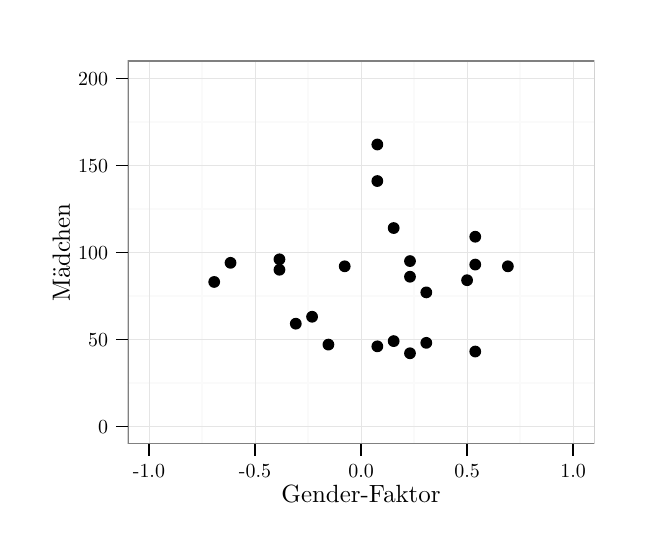
\begin{tikzpicture}[x=1pt,y=1pt]
\definecolor[named]{fillColor}{rgb}{1.00,1.00,1.00}
\path[use as bounding box,fill=fillColor,fill opacity=0.00] (0,0) rectangle (216.81,180.67);
\begin{scope}
\path[clip] (  0.00,  0.00) rectangle (216.81,180.67);
\definecolor[named]{drawColor}{rgb}{1.00,1.00,1.00}
\definecolor[named]{fillColor}{rgb}{1.00,1.00,1.00}

\path[draw=drawColor,line width= 0.6pt,line join=round,line cap=round,fill=fillColor] (  0.00,  0.00) rectangle (216.81,180.67);
\end{scope}
\begin{scope}
\path[clip] ( 36.15, 30.32) rectangle (204.76,168.63);
\definecolor[named]{fillColor}{rgb}{1.00,1.00,1.00}

\path[fill=fillColor] ( 36.15, 30.32) rectangle (204.76,168.63);
\definecolor[named]{drawColor}{rgb}{0.98,0.98,0.98}

\path[draw=drawColor,line width= 0.6pt,line join=round] ( 36.15, 52.32) --
	(204.76, 52.32);

\path[draw=drawColor,line width= 0.6pt,line join=round] ( 36.15, 83.76) --
	(204.76, 83.76);

\path[draw=drawColor,line width= 0.6pt,line join=round] ( 36.15,115.19) --
	(204.76,115.19);

\path[draw=drawColor,line width= 0.6pt,line join=round] ( 36.15,146.63) --
	(204.76,146.63);

\path[draw=drawColor,line width= 0.6pt,line join=round] ( 62.98, 30.32) --
	( 62.98,168.63);

\path[draw=drawColor,line width= 0.6pt,line join=round] (101.30, 30.32) --
	(101.30,168.63);

\path[draw=drawColor,line width= 0.6pt,line join=round] (139.62, 30.32) --
	(139.62,168.63);

\path[draw=drawColor,line width= 0.6pt,line join=round] (177.94, 30.32) --
	(177.94,168.63);
\definecolor[named]{drawColor}{rgb}{0.90,0.90,0.90}

\path[draw=drawColor,line width= 0.2pt,line join=round] ( 36.15, 36.60) --
	(204.76, 36.60);

\path[draw=drawColor,line width= 0.2pt,line join=round] ( 36.15, 68.04) --
	(204.76, 68.04);

\path[draw=drawColor,line width= 0.2pt,line join=round] ( 36.15, 99.47) --
	(204.76, 99.47);

\path[draw=drawColor,line width= 0.2pt,line join=round] ( 36.15,130.91) --
	(204.76,130.91);

\path[draw=drawColor,line width= 0.2pt,line join=round] ( 36.15,162.34) --
	(204.76,162.34);

\path[draw=drawColor,line width= 0.2pt,line join=round] ( 43.82, 30.32) --
	( 43.82,168.63);

\path[draw=drawColor,line width= 0.2pt,line join=round] ( 82.14, 30.32) --
	( 82.14,168.63);

\path[draw=drawColor,line width= 0.2pt,line join=round] (120.46, 30.32) --
	(120.46,168.63);

\path[draw=drawColor,line width= 0.2pt,line join=round] (158.78, 30.32) --
	(158.78,168.63);

\path[draw=drawColor,line width= 0.2pt,line join=round] (197.10, 30.32) --
	(197.10,168.63);
\definecolor[named]{fillColor}{rgb}{0.00,0.00,0.00}

\path[fill=fillColor] (108.67, 66.15) circle (  2.13);

\path[fill=fillColor] (114.56, 94.44) circle (  2.13);

\path[fill=fillColor] (126.35, 65.52) circle (  2.13);

\path[fill=fillColor] (126.35,138.45) circle (  2.13);

\path[fill=fillColor] (138.15, 63.01) circle (  2.13);

\path[fill=fillColor] (161.73,105.13) circle (  2.13);

\path[fill=fillColor] ( 73.30, 95.70) circle (  2.13);

\path[fill=fillColor] ( 90.98, 96.96) circle (  2.13);

\path[fill=fillColor] ( 90.98, 93.19) circle (  2.13);

\path[fill=fillColor] (173.52, 94.44) circle (  2.13);

\path[fill=fillColor] ( 67.40, 88.78) circle (  2.13);

\path[fill=fillColor] ( 96.88, 73.70) circle (  2.13);

\path[fill=fillColor] (102.77, 76.21) circle (  2.13);

\path[fill=fillColor] (126.35,125.25) circle (  2.13);

\path[fill=fillColor] (132.25,108.27) circle (  2.13);

\path[fill=fillColor] (132.25, 67.41) circle (  2.13);

\path[fill=fillColor] (161.73, 63.64) circle (  2.13);

\path[fill=fillColor] (144.04, 66.78) circle (  2.13);

\path[fill=fillColor] (138.15, 96.33) circle (  2.13);

\path[fill=fillColor] (138.15, 90.67) circle (  2.13);

\path[fill=fillColor] (144.04, 85.01) circle (  2.13);

\path[fill=fillColor] (158.78, 89.41) circle (  2.13);

\path[fill=fillColor] (161.73, 95.07) circle (  2.13);
\definecolor[named]{drawColor}{rgb}{0.50,0.50,0.50}

\path[draw=drawColor,line width= 0.6pt,line join=round,line cap=round] ( 36.15, 30.32) rectangle (204.76,168.63);
\end{scope}
\begin{scope}
\path[clip] (  0.00,  0.00) rectangle (216.81,180.67);
\definecolor[named]{drawColor}{rgb}{0.00,0.00,0.00}

\node[text=drawColor,anchor=base east,inner sep=0pt, outer sep=0pt, scale=  0.72] at ( 29.04, 34.12) {0};

\node[text=drawColor,anchor=base east,inner sep=0pt, outer sep=0pt, scale=  0.72] at ( 29.04, 65.56) {50};

\node[text=drawColor,anchor=base east,inner sep=0pt, outer sep=0pt, scale=  0.72] at ( 29.04, 96.99) {100};

\node[text=drawColor,anchor=base east,inner sep=0pt, outer sep=0pt, scale=  0.72] at ( 29.04,128.43) {150};

\node[text=drawColor,anchor=base east,inner sep=0pt, outer sep=0pt, scale=  0.72] at ( 29.04,159.86) {200};
\end{scope}
\begin{scope}
\path[clip] (  0.00,  0.00) rectangle (216.81,180.67);
\definecolor[named]{drawColor}{rgb}{0.00,0.00,0.00}

\path[draw=drawColor,line width= 0.6pt,line join=round] ( 31.89, 36.60) --
	( 36.15, 36.60);

\path[draw=drawColor,line width= 0.6pt,line join=round] ( 31.89, 68.04) --
	( 36.15, 68.04);

\path[draw=drawColor,line width= 0.6pt,line join=round] ( 31.89, 99.47) --
	( 36.15, 99.47);

\path[draw=drawColor,line width= 0.6pt,line join=round] ( 31.89,130.91) --
	( 36.15,130.91);

\path[draw=drawColor,line width= 0.6pt,line join=round] ( 31.89,162.34) --
	( 36.15,162.34);
\end{scope}
\begin{scope}
\path[clip] (  0.00,  0.00) rectangle (216.81,180.67);
\definecolor[named]{drawColor}{rgb}{0.00,0.00,0.00}

\path[draw=drawColor,line width= 0.6pt,line join=round] ( 43.82, 26.05) --
	( 43.82, 30.32);

\path[draw=drawColor,line width= 0.6pt,line join=round] ( 82.14, 26.05) --
	( 82.14, 30.32);

\path[draw=drawColor,line width= 0.6pt,line join=round] (120.46, 26.05) --
	(120.46, 30.32);

\path[draw=drawColor,line width= 0.6pt,line join=round] (158.78, 26.05) --
	(158.78, 30.32);

\path[draw=drawColor,line width= 0.6pt,line join=round] (197.10, 26.05) --
	(197.10, 30.32);
\end{scope}
\begin{scope}
\path[clip] (  0.00,  0.00) rectangle (216.81,180.67);
\definecolor[named]{drawColor}{rgb}{0.00,0.00,0.00}

\node[text=drawColor,anchor=base,inner sep=0pt, outer sep=0pt, scale=  0.72] at ( 43.82, 18.24) {-1.0};

\node[text=drawColor,anchor=base,inner sep=0pt, outer sep=0pt, scale=  0.72] at ( 82.14, 18.24) {-0.5};

\node[text=drawColor,anchor=base,inner sep=0pt, outer sep=0pt, scale=  0.72] at (120.46, 18.24) {0.0};

\node[text=drawColor,anchor=base,inner sep=0pt, outer sep=0pt, scale=  0.72] at (158.78, 18.24) {0.5};

\node[text=drawColor,anchor=base,inner sep=0pt, outer sep=0pt, scale=  0.72] at (197.10, 18.24) {1.0};
\end{scope}
\begin{scope}
\path[clip] (  0.00,  0.00) rectangle (216.81,180.67);
\definecolor[named]{drawColor}{rgb}{0.00,0.00,0.00}

\node[text=drawColor,anchor=base,inner sep=0pt, outer sep=0pt, scale=  0.90] at (120.46,  9.03) {Gender-Faktor};
\end{scope}
\begin{scope}
\path[clip] (  0.00,  0.00) rectangle (216.81,180.67);
\definecolor[named]{drawColor}{rgb}{0.00,0.00,0.00}

\node[text=drawColor,rotate= 90.00,anchor=base,inner sep=0pt, outer sep=0pt, scale=  0.90] at ( 15.23, 99.47) {Mädchen};
\end{scope}
\end{tikzpicture}
